\chapter{Environment}
\label{chapter:environment}

\section{Extending JUnit for Spring Framework domain}
    \textbf{Spring} is a framework for Java, described as:
    \textit{"core support for dependency injection, transaction management, web applications, data access, messaging, testing and more."}~\cite{spring}
    It is targeted for Java enterprise applications, providing teams with a framework that allows them to primarily focus on
    application's business logic~\cite{spring}. Spring framework ships with a lot modules and features that needs to be
    configured for the project~\cite{wiki:spring}. \textbf{Spring Boot} is \textit{convention-over-configuration} solution
    composed of the Spring Framework components, that enables rapid application development with minimal effort to get started~\cite{wiki:spring}.

    Spring Framework integration testing can be done by extending JUnit with custom Spring JUnit runner class or by using Spring JUnit class and
    method rules. Runner class and the Spring JUnit rules both provide standard Spring test context
    for integration tests with features such as dependency injection and transactional test method execution. ~\cite{springintegration}

    \begin{figure}[ht]
      \begin{center}
        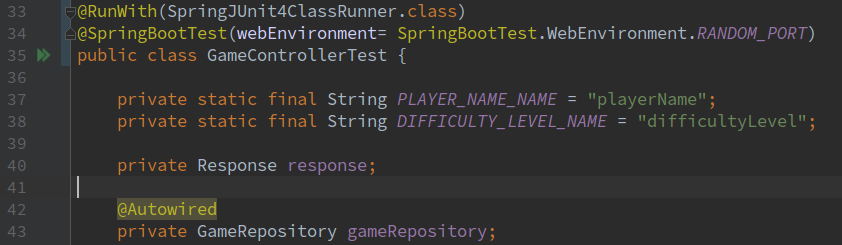
\includegraphics[width=13.5cm]{images/springrunner.png}
        \caption{JUnit extended for Spring integration testing}
        \label{fig:springrunner}
      \end{center}
    \end{figure}

    Figure \ref{fig:springrunner} shows example of a Spring Boot JUnit integration test, where the context and its configuration are
    loaded with lines 33 and 34. Line 33. is an example of extending JUnit with custom runner. Lines 42-43 show example of injected dependency
    via Spring Framework.

    JUnit and its extensions provide a base for automated low level testing of Java-code.
    In the next section alternatives for Java-code testing are presented with implementation level BDD testing frameworks from
    various JVM programming languages.

\section{Implementation level BDD testing frameworks for JVM}
    As this thesis is interested in testing Java-code, the scope of implementation level BDD is limited to testing frameworks
    found from JVM programming languages. As stated before, these languages hold ones such as \textit{Ruby, Groovy, Python,
    Clojure} and \textit{Scala}. Through all these languages there exists many alternatives for both implementation and
    acceptance level BDD testing frameworks. For implementation level, there exists two alternative approaches to practicing
    BDD: \textbf{xSpec family}~\cite{solis2011study} and \textbf{Gherkin family} testing frameworks.

    \subsection{xSpec family}
    xSpec family testing frameworks are restricted to implementation level~\cite{solis2011study}. xSpec style testing
    is examined in more detail in this section through \textbf{RSpec} via JRuby, but it also demonstrated with
    Java 8 -based \textbf{Spectrum}. There exists also other possibilities for xSpec family testing in JVM enviroment,
    for example Scala-based \textbf{FunSpec}~\cite{funspec} for ScalaTest, but they are not examined in detail.
    \subsubsection{RSpec}
    Ruby community has been for a long time a steady advocate of TDD~\cite{lerner2009forge}. It is also the birth place
    of first implementation level BDD testing framework: \textbf{RSpec}~\cite{astels2006new}. Whereas first BDD framework
    JBehave~\cite{bdd2006north} was aimed for acceptance level and all stakeholders, RSpec brought the behavior driven thinking for developer
    audience~\cite{astels2006new}.

    RSpec is the founding framework in xSpec family of testing. In its current version 3.5, it is a mature holistic testing
    framework including \textit{expectations} library (assertions), \textit{mocking capabilities, integrations} to Ruby frameworks and the \textit{core runner}~\cite{rspecdoc}.
    In the next chapter RSpec usage for testing Java-code both at unit and integration level for Spring framework is reviewed,
    but before this, the core concepts of RSpec are illustrated.

    The main functionality of RSpec comes from the core runner. It includes the code \textbf{example groups} that can hold runnable
    specification \textbf{code examples}~\cite{chelimsky2010rspec}. These examples and groups are created into a \textbf{spec} file~\cite{chelimsky2010rspec}.
    Example groups can be initialized with keywords \textit{describe}
    and \textit{context}, which both are aliases for each other~\cite{rspec-core}. Example groups can inherit each other nested in a single
    file, creating nested context groups~\cite{rspec-core}. This can help immensively on removing repetition from the test code
    and achieving easily readable test outputs~\cite{chelimsky2010rspec}.

    Specification code examples can be created with the keywords \textit{it, specify} and \textit{example}~\cite{rspec-core}.
    These examples create executable pieces of behavior of the code under specification~\cite{chelimsky2010rspec}. Code examples
    contain \textbf{expectations}, which specify the expected behavior of the given example~\cite{chelimsky2010rspec}. Expectations can
    be seen as assertions from xUnit testing family, but the reason for changing the language is to support better communication
    between stakeholders, in this case developers~\cite{chelimsky2010rspec}. As BDD is an evolution of TDD, expectations
    was created to establish a better language for what the code to be developed \textit{should} do, instead of verifying it
    with assertions~\cite{astels2006new}. The guideline is for the code examples to hold only one expectation per example~\cite{chelimsky2010rspec}.
    This allows separate info about failing situations~\cite{chelimsky2010rspec} and provides a rule \textbf{one assert per test method}
    for living specification~\cite{astels2006new}. This rule was originally created by Astels~\cite{astels2006new} to
    help TDD practitioners to change viewpoint from 1-1 relationship between test classes and methods to production classes
    and methods.

    Examples of RSpec spec files are introduced in the next chapter.
    The following table shows the relationships between RSpec testing terms compared to xUnit architecture components~\cite{chelimsky2010rspec}:
    \begin{longtable}{@{}p{0.25\textwidth}p{0.7\textwidth}@{}}
    Expectations & \Longrightarrow  \textrm{Assertions} \\
    Code Example & \Longrightarrow  \textrm{Test Method} \\
    Example Group & \Longrightarrow  \textrm{Test Case} \\
    Spec File & \Longrightarrow  \textrm{Test Suite} \\
    \end{longtable}

    \subsubsection{Spectrum}

    \subsection{Gherkin family}
    Gherkin family is a term defined in this thesis, containing BDD testing frameworks that use predetermined ubiquitous
    language \textbf{Gherkin}~\cite{gherkin}. There exists research related to usage of Gherkin in BDD testing frameworks~\cite{okolnychyi2016study}.
    Gherkin family frameworks exists for both acceptance and implementation testing level~\cite{okolnychyi2016study}. For Java-code testing at
    implementation level with Gherkin, JVM offers for example \textbf{Spock}~\cite{spock} via Groovy, Java 8 -based \textbf{Spectrum}~\cite{spectrum},
    JRuby-based \textbf{RSpec-given}~\cite{rspec-given} for Rspec and Scala-based \textbf{FeatureSpec}~\cite{featurespec} for ScalaTest.
    Spock will be used as an example for inspecting implementation level testing with a Gherkin family framework.
    \subsubsection{Spock}
    \textbf{Spock} is a BDD testing framework for JVM programming language Groovy~\cite{kapelonis2016java}. It supports
    testing both Java and Groovy code and it can be considered a superset of JUnit, as it extends the JUnit runner~\cite{spock}.
    As a result of this, it is considered "enterprise ready" with \textit{support for IDEs, JUnit rules, external tools} that use
    JUnit runner and easy \textit{build tool integrations}~\cite{kapelonis2016java}.
    Spock is capable of testing the whole automated BDD cycle from acceptance level to unit level~\cite{kapelonis2016java}.
    It holds unit test support with integrated mocking and stubbing capabilities and integration testing support with extending it for
    example Spring Framework~\cite{kapelonis2016java}. Spock also supports Data Driven Testing with tabular format readable DSL~\cite{spock}.
    Data Driven Testing can drastically remove repetition from test code and makes it easier to test different parameter
    variations~\cite{kapelonis2016java}. Figure \ref{fig:spock-debug} displays console debugger of Spock related to
    condition checking. This display of objects and their values and the assertion checks straight in the console
    can reduce the need for explicit debugging~\cite{kapelonis2016java}.
    \begin{figure}[ht]
      \begin{center}
        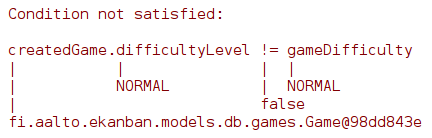
\includegraphics[width=9.5cm]{images/spock-debug.png}
        \caption{Spock console debugger}
        \label{fig:spock-debug}
      \end{center}
    \end{figure}

    As stated earlier, Spock is a BDD testing framework with Gherkin support.
    Full functionality of Gherkin includes feature and scenario information described
    with \textbf{Given-When-Then} steps for plain text test input~\cite{gherkin}. This makes it easier for stakeholder collaboration
    and is aimed at acceptance testing level.
    Spock supports full Gherkin through additional library \textit{Pease}, but the support for it is deprecated~\cite{spock-pease}.
    Although Spock can be configured to use plain text Gherkin, its normal usage is aimed for developer audience at implementation
    level with test code and Gherkin descriptions mixed in together~\cite{okolnychyi2016study}.

    Spock terminology consists of \textbf{specification} files containing \textbf{feature methods} and Given-When-Then
    \textbf{blocks} inside them~\cite{spock}. Examples of Spock specification files can be found in the next chapter
    when its setup for a Gradle project is demonstrated.
    Spock makes heavy use of Gherkin's Given-When-Then with runnable code blocks for each steps, that can contain textual
    description~\cite{kapelonis2016java}:
    \begin{itemize}
    \item \textbf{Given} is a code block used to initialize the context of test
    \item \textbf{When} is a code block used to trigger the action, stimulus of the test
    \item \textbf{Then} is a code block containing power assertions to verify \textbf{conditions}
    \end{itemize}
    JUnit testing literature also states to use this kind of structure with \textbf{Arrange-Act-Assert (AAA)},
    where different parts are separated from each other with space between them~\cite{langr2015pragmatic}.
    As this structure is not enforced in JUnit, there is the considerable possibility that it will not be used~\cite{kapelonis2016java}.


